\chapter{Appendix E: Parameter Values Used}
\label{AppendixE}

\section{Realistic Growth Curves}
\label{sec:appendixE:a_good_curve}
\begin{table}[ht!]
    \small % or \footnotesize to make it more compact
    \centering
    \begin{tabularx}{\textwidth}{l l l l}
        \toprule
        IC\\
        \textbf{Resources} & \textbf{Uninfected Bacteria} & \textbf{Infected Bacteria} & \textbf{Phages} \\
        \midrule
        400 & 50 & \scalebox{1}{$
            \begin{bmatrix}
                0 & 0 & 0 & 0 \\
            \end{bmatrix}
        $} & 10 \\
        \bottomrule
    \end{tabularx}\newline
    \begin{tabularx}{\textwidth}{l l}
        \toprule
        Vector Data\\
        \bm{$\tau$} & \bm{$\omega^i$}\\
        \midrule
        2.14 & 0 \\
        \bottomrule
    \end{tabularx}\newline
    \begin{tabularx}{\textwidth}{l l l l l}
        \toprule
        Matrix Data\\
        \bm{$e$} & \bm{$v$} & \bm{$K$} & \bm{$r$} & \bm{$\beta$} \\
        \midrule
        0.03 & 1.2 & 10 & 0.01 & 20 \\
        \bottomrule
    \end{tabularx}\newline
    \begin{tabularx}{\textwidth}{l l}
        \toprule
        Environment Data\\
        \bm{$M$} & \bm{$\omega^o$}\\
        \midrule
        4 & 0 \\
        \bottomrule
    \end{tabularx}\newline
    \caption{
        The parameter values used for \Cref{fig:created:a_good_curve}. 
    }
    \label{tab:appendixE:a_good_curve}
\end{table}

\section{A Second Realistic Growth Curve}
\label{sec:appendixE:a_good_curve_2}

\begin{figure}[ht!]
    \centering
    \begin{subfigure}{1\linewidth}
        \centering
        \captionsetup{width=1\linewidth}
        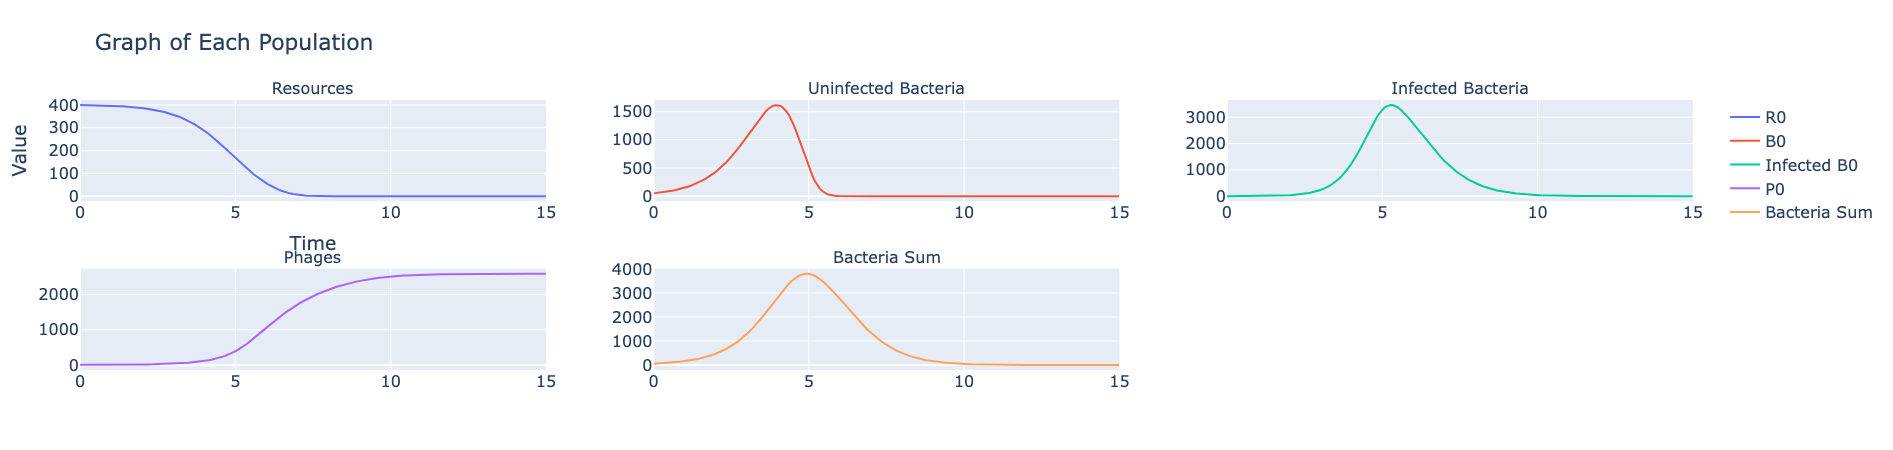
\includegraphics[width=\linewidth]{Plots/Created/a_good_curve_linear.png}
        \caption{
            A second realistic growth curve, linear y-axis
        }
        \label{fig:created:a_good_curve_linear_2}
    \end{subfigure}
    \hfill
    \begin{subfigure}{1\linewidth}
        \centering
        \captionsetup{width=1\linewidth}
        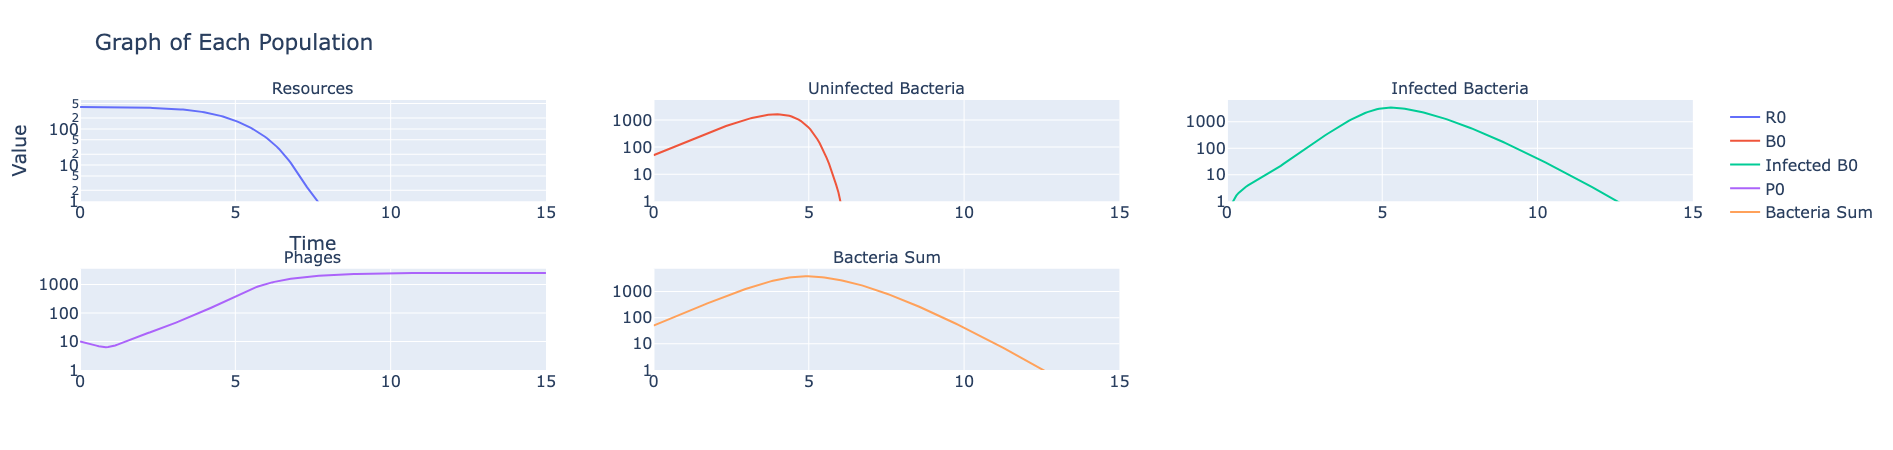
\includegraphics[width=\linewidth]{Plots/Created/a_good_curve_logarithmic.png}
        \caption{
            A second realsitic growth curve, logarithmic y-axis. 
        }
        \label{fig:created:a_good_curve_logarithmic_2}
    \end{subfigure}
    \caption{
        The parameters used for this plot can be found in \Cref{tab:appendixE:a_good_curve}. 
    }
    \label{fig:created:a_good_curve_2}
\end{figure}

\begin{table}[ht!]
    \small % or \footnotesize to make it more compact
    \centering
    \begin{tabularx}{\textwidth}{l l l l}
        \toprule
        IC\\
        \textbf{Resources} & \textbf{Uninfected Bacteria} & \textbf{Infected Bacteria} & \textbf{Phages} \\
        \midrule
        200 & 50 & \scalebox{1}{$
            \begin{bmatrix}
                0 & 0 & 0 & 0 \\
            \end{bmatrix}
        $} & 10 \\
        \bottomrule
    \end{tabularx}\newline
    \begin{tabularx}{\textwidth}{l l}
        \toprule
        Vector Data\\
        \bm{$\tau$} & \bm{$\omega^i$}\\
        \midrule
        0.7 & 0 \\
        \bottomrule
    \end{tabularx}\newline
    \begin{tabularx}{\textwidth}{l l l l l}
        \toprule
        Matrix Data\\
        \bm{$e$} & \bm{$v$} & \bm{$K$} & \bm{$r$} & \bm{$\beta$} \\
        \midrule
        0.12 & 1 & 10 & 0.001 & 10 \\
        \bottomrule
    \end{tabularx}\newline
    \begin{tabularx}{\textwidth}{l l}
        \toprule
        Environment Data\\
        \bm{$M$} & \bm{$\omega^o$}\\
        \midrule
        4 & 0 \\
        \bottomrule
    \end{tabularx}\newline
    \caption{
        Another set of realistic growth curves. 
        The linear and logarithmic plot of this data can be seen in \Cref{fig:created:a_good_curve_2}
    }
    \label{tab:appendixE:a_good_curve_2}
\end{table}

\section{SOBOL Analysis}
\begin{table}[ht!]
    \small % or \footnotesize to make it more compact
    \centering
    \begin{tabularx}{\textwidth}{l l l}
        \toprule
        IC\\
        \textbf{Resources} & \textbf{Uninfected Bacteria} & \textbf{Phages} \\
        \midrule
        1-500 & 1-100 & 1-50 \\ 
        \bottomrule
    \end{tabularx}\newline
    \begin{tabularx}{\textwidth}{l l}
        \toprule
        Vector Data\\
        \bm{$\tau$} & \bm{$\omega^i$}\\
        \midrule
        0.5-3.5 & 0-100 \\
        \bottomrule
    \end{tabularx}\newline
    \begin{tabularx}{\textwidth}{l l l l l}
        \toprule
        Matrix Data\\
        \bm{$e$} & \bm{$v$} & \bm{$K$} & \bm{$r$} & \bm{$\beta$} \\
        \midrule
        0.05-0.25 & 0.8-1.9 & 10-250 & 0.001-0.2 & 1-100 \\
        \bottomrule
    \end{tabularx}\newline
    \begin{tabularx}{\textwidth}{l}
        \toprule
        Environment Data\\
        \bm{$\omega^o$}\\
        \midrule
        0-0.1 \\
        \bottomrule
    \end{tabularx}\newline
    \begin{tabularx}{\textwidth}{l l l l l}
        \toprule
        Other Data\\
        \textbf{Seed Value} & \textbf{2nd Order} & \textbf{Number Samples} & \textbf{Simulations Run} & \textbf{Simulation Length}\\
        \midrule
        0 & False & 15 & $2^{15}(9+2) = 360448$ & 15\\
        \bottomrule
    \end{tabularx}\newline
    \caption{
        The parameter values used for the SOBOL sensitivity analysis in \Cref{fig:created:SOBOL_no_wi_wo} (SOBOL analysis without washin and washout) and \Cref{fig:created:SOBOL_analyses} (SOBOL analysis with washin and washout). 
        For SOBOL analysis with washin and washout, there are $2^{15}(9+2) = 425984$ unique simulations run. 
    }
    \label{tab:appendixE:SOBOL_analysis_values}
\end{table}

\section{Complex Model}
\label{sec:appendixE:complex_model}
\begin{table}[ht!]
    \small % or \footnotesize to make it more compact
    \centering
    \begin{tabularx}{\textwidth}{l l l l}
        \toprule
        IC\\
        \textbf{Resources} & \textbf{Uninfected Bacteria} & \textbf{Infected Bacteria} & \textbf{Phages} \\
        \midrule
        \scalebox{1}{$
            \begin{bmatrix}
                236 & 287 & 270 \\
            \end{bmatrix}
        $} & 
        \scalebox{1}{$
            \begin{bmatrix}
                53 & 69 \\
            \end{bmatrix}
        $} & 
        \scalebox{1}{$
            \begin{bmatrix}
                0 & 0 & 0 & 0 \\
                0 & 0 & 0 & 0 \\
            \end{bmatrix}
        $} & 
        \scalebox{1}{$
            \begin{bmatrix}
                10 & 5 & 8 \\
            \end{bmatrix}
        $} \\
        \bottomrule
    \end{tabularx}\newline
    \begin{tabularx}{\textwidth}{l l}
        \toprule
        Vector Data\\
        \bm{$\tau_b$} & \bm{$\omega^i_r$} \\
        \midrule
        \scalebox{1}{$
            \begin{bmatrix}
                2.73340 & 2.25015 \\
            \end{bmatrix}
        $} & 
        \scalebox{1}{$
            \begin{bmatrix}
                0 & 0 & 0 \\
            \end{bmatrix}
        $} \\
        \bottomrule
    \end{tabularx}\newline
    \begin{tabularx}{\textwidth}{l l}
        \toprule
        Matrix Data\\
        \bm{$e_{b r}$} & \bm{$v_{b r}$} \\
        \midrule
        \scalebox{1}{$
            \begin{bmatrix}
                0.15680 & 0.10871 & 0 \\
                0 & 0 & 0.18009 \\
            \end{bmatrix}
        $} & 
        \scalebox{1}{$
            \begin{bmatrix}
                1.27601 & 0.86393 & 0 \\
                0 & 0 & 1.22625 \\
            \end{bmatrix}
        $} \\
        \bottomrule
    \end{tabularx}\newline
    \begin{tabularx}{\textwidth}{l l l}
        \bm{$K_{b r}$} & \bm{$r_{p b}$} & \bm{$\beta_{p b}$} \\
        \midrule
        \scalebox{1}{$
            \begin{bmatrix}
                139.58353 & 12.83058 & 0 \\
                0 & 0 & 82.86684 \\
            \end{bmatrix}
        $} & 
        \scalebox{1}{$
            \begin{bmatrix}
                0 & 0.11695 \\
                0.144459 & 0 \\
                0.11895 & 0.13065 \\
            \end{bmatrix}
        $} & 
        \scalebox{1}{$
            \begin{bmatrix}
                0 & 15 \\
                34 & 0 \\
                11 & 57 \\
            \end{bmatrix}
        $}\\
        \bottomrule
    \end{tabularx}\newline
    \begin{tabularx}{\textwidth}{l l}
        \toprule
        Environment Data\\
        \bm{$M$} & \bm{$\omega^o$}\\
        \midrule
        4 & 0 \\
        \bottomrule
    \end{tabularx}\newline
    \caption{
        The parameter values used for the $3\times2\times3$ network model rounded to 5 decimal points. 
        If there is no edge between a phage, bacteria, or resource, then in the matrix representation of the parameter, 0 is stored as the default value. 
    }
    \label{tab:appendixE:complex_model}
\end{table}